\section{Results}
\label{sec:results}

\subsection{E1: Over-exposure}
\label{sec:res-exposure}
Table~\ref{tab:e1} and Fig.~\ref{fig:e1} report scope-level results on all \nTasks{} permitted tasks. Under the full
entitlement (B0, and equally B2 and B3, whose reach is $E(u)$) an agent can reach \oerColBzero{} times as many columns
as the gold query needs (geometric mean) and \oerCellBzero{} times as many cells. Static role views (B1) reduce this to
\oerColBone{} and \oerCellBone{}. The default TSE scope reaches \oerColTse{} times the needed columns and \oerCellTse{}
times the needed cells, a \oerColReduction-fold reduction in columns and a \oerCellReduction-fold reduction in cells
relative to B0. TSE is lower than both B0 and B1 on every granularity and dataset (Table~\ref{tab:e1tests}; all
Holm-adjusted $p\le\eoneMaxPHolm$). Row-level over-exposure falls less (\oerRowBzero{} to \oerRowTse{}) because task
filters are only kept when grounded in the task text and $k{=}1$ drops range filters. The reduction is robust to the
policy generator: across nine seed and fraction settings the column-level reduction ranges from
\sensRatioMin{}$\times$ to \sensRatioMax{}$\times$ (Table~\ref{tab:sens}). \emph{Takeaway: per task, an agent under TSE
can reach a small fraction of the data its user can reach.}

\begin{figure}[t]
\centering
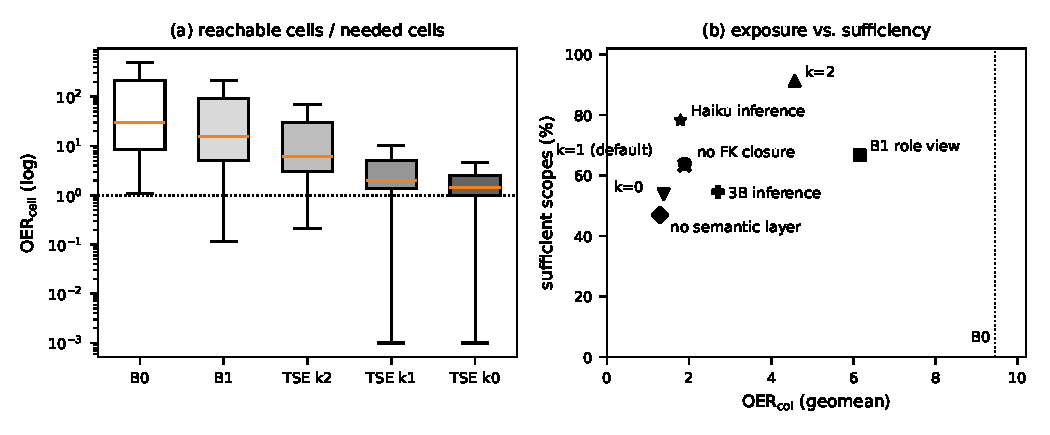
\includegraphics[width=\columnwidth]{figs/fig_e1.pdf}
\caption{(a) Cell-level over-exposure per task (log scale; 1 = only needed data reachable). (b) Exposure versus
sufficiency for TSE variants; the dotted line marks B0. Synthetic-policy entitlements.}
\label{fig:e1}
\end{figure}

\begin{table*}[t]\centering\caption{Scope-level results on all permitted tasks (E1, E3). OER: geometric mean over tasks (1 = only needed data reachable). Sufficiency: the gold query, executed under the compiled scope, returns the gold result (95\% bootstrap CI). Column precision/recall against the gold scope $N(t)$. Synthetic-policy entitlements.}\label{tab:e1}
\footnotesize\begin{tabular}{lrrrrrrr}\hline
\textbf{Scope source} & \textbf{OER$_\mathrm{col}$} & \textbf{OER$_\mathrm{row}$} & \textbf{OER$_\mathrm{cell}$} & \textbf{Sufficient (\%)} & \textbf{Col.\ prec.} & \textbf{Col.\ rec.} & \textbf{Median cols} \\\hline
B0 / B2 / B3 (reach $=E(u)$) & 9.45 & 2.67 & 50.6 & 100.0 [100.0, 100.0] & 0.15 & 1.00 & 31 \\
B1 static role view & 6.16 & 1.81 & 28.8 & 66.7 [63.8, 69.6] & 0.18 & 0.89 & 25 \\
TSE $k{=}0$ & 1.38 & 0.40 & 1.1 & 53.8 [50.7, 56.8] & 0.69 & 0.90 & 5 \\
TSE $k{=}1$ (default) & 1.90 & 0.60 & 2.1 & 63.9 [60.9, 66.9] & 0.55 & 0.94 & 7 \\
TSE $k{=}2$ & 4.57 & 2.47 & 13.2 & 91.3 [89.5, 93.0] & 0.28 & 0.98 & 16 \\
TSE no FK closure & 1.89 & 0.59 & 2.1 & 63.3 [60.3, 66.3] & 0.55 & 0.94 & 7 \\
TSE no semantic layer & 1.29 & 0.42 & 1.2 & 47.0 [43.9, 50.1] & 0.62 & 0.86 & 5 \\
TSE small inference model & 2.71 & 0.36 & 4.9 & 54.6 [51.5, 57.7] & 0.40 & 0.91 & 9 \\
TSE Haiku-5.5 inference (exploratory) & 1.79 & 0.85 & 2.1 & 78.2 [75.7, 80.7] & 0.57 & 0.97 & 7 \\
\hline\end{tabular}\end{table*}

\begin{table}[t]\centering\caption{E1 paired Wilcoxon signed-rank tests, TSE vs.\ baseline ($n$ excludes tied pairs, which the test drops; Holm-adjusted $p$; effect size: matched-pairs rank-biserial $r$, negative = TSE lower).}\label{tab:e1tests}
\footnotesize\begin{tabular}{llllrr}\hline
\textbf{Data} & \textbf{OER} & \textbf{vs.} & $n$ & $r$ & $p_\mathrm{Holm}$ \\\hline
bird & col & B0 & 488 & -1.00 & $<10^{-6}$ \\
bird & col & B1 & 488 & -0.99 & $<10^{-6}$ \\
bird & row & B0 & 340 & -1.00 & $<10^{-6}$ \\
bird & row & B1 & 346 & -0.94 & $<10^{-6}$ \\
bird & cell & B0 & 500 & -1.00 & $<10^{-6}$ \\
bird & cell & B1 & 500 & -0.99 & $<10^{-6}$ \\
spider & col & B0 & 500 & -1.00 & $<10^{-6}$ \\
spider & col & B1 & 496 & -0.99 & $<10^{-6}$ \\
spider & row & B0 & 155 & -1.00 & $<10^{-6}$ \\
spider & row & B1 & 180 & -0.77 & $<10^{-6}$ \\
spider & cell & B0 & 500 & -1.00 & $<10^{-6}$ \\
spider & cell & B1 & 500 & -0.98 & $<10^{-6}$ \\
\hline\end{tabular}\end{table}


\subsection{E3: Scope-inference quality}
\label{sec:res-inference}
Inference quality is the load-bearing assumption. The default scope is sufficient on \suffTse\% of tasks
(95\% CI [\suffLoTse, \suffHiTse]; \suffTseBird\% on BIRD and \suffTseSpider\% on Spider), with mean column recall
\recTse{} and precision \precTse{}. The gold scope $N(t)$ itself is sufficient on \goldSufficient\% of tasks, which
validates the extraction. Conservativeness behaves monotonically: $k{=}0$ is sufficient on \suffTsekzero\% at
OER$_\mathrm{col}$ \oerColTsekzero{}, $k{=}2$ on \suffTsektwo\% at \oerColTsektwo{}. Removing FK closure lowers
sufficiency to \suffTsenoclose\%; removing the semantic layer (no descriptions, no linking) to \suffTsenosl\%; a 3B
inference model reaches \suffTsesmall\%. As an exploratory comparison, Claude Haiku 5.5 as inference model reaches
\suffTsehaiku\%. In a random sample of \taxN{} insufficient scopes, the causes were: a needed non-key column was missing (50\%); a task row filter excluded needed rows (30\%); a needed table was missing (11\%); the query was rejected through views (9\%) (taxonomy table in the supplementary material).


\subsection{E2: Utility}
\label{sec:res-utility}
Table~\ref{tab:e2} reports execution accuracy. For Claude Haiku 5.5, B0 reaches \exHaikuBzero\%, B3 \exHaikuBthree\%,
and TSE \exHaikuTse\% (paired difference to B0: \dExHaikuTse{} pp, 95\% CI [\dExLoHaikuTse, \dExHiHaikuTse]). For
Claude Sonnet 5.5 the corresponding values are \exSonnetBzero\%, \exSonnetBthree\% and \exSonnetTse\% (\dExSonnetTse{}
pp, [\dExLoSonnetTse, \dExHiSonnetTse]). Static role views (B1) cost the most: \dExHaikuBone{} pp for Haiku 5.5, because
a role-level view built from other tasks misses columns that a new task needs. Agents under TSE requested widening in
\wreqHaiku\% of runs (Haiku 5.5) and \wreqSonnet\% (Sonnet 5.5); at least one request was approved in \wappHaiku\% and
\wappSonnet\% of runs. 


\textbf{Conservativeness and widening policy (exploratory).} On a \ablN-task subset (Haiku 5.5,
Table~\ref{tab:ablation}), where B0 reaches \ablExBzero\% and default TSE \ablExDefault\%, a narrower scope ($k{=}0$)
lowers execution accuracy by \ablDKzero{} pp ([\ablDLoKzero, \ablDHiKzero]) and a broader one ($k{=}2$) raises it by
\ablDKtwo{} pp ([\ablDLoKtwo, \ablDHiKtwo]) to \ablExKtwo\%, close to B0, while widening requests drop to
\ablWreqKtwo\% of runs. $k$ therefore trades exposure (Section~\ref{sec:res-inference}) for utility directly. The
\emph{strict} policy changes accuracy by \ablDStrict{} pp ([\ablDLoStrict, \ablDHiStrict]); denying all widening
costs \ablDDeny{} pp ([\ablDLoDeny, \ablDHiDeny]). Across \seedReps{} independent repetitions on \seedSubsetN{}
tasks, B0 ranged from \seedExBzeroMin\% to \seedExBzeroMax\% and TSE from \seedExTseMin\% to \seedExTseMax\%; the TSE
minus B0 difference ranged from \seedDiffMin{} to \seedDiffMax{} pp.

\begin{table}[t]\centering\caption{Agent-level ablations (Haiku 5.5, both harnesses, 200 permitted tasks). $\Delta$: paired EX difference to default TSE ($k{=}1$, \emph{auto}) on the same tasks (95\% CI). Exploratory.}\label{tab:ablation}
\footnotesize\begin{tabular}{lrrlr}\hline\textbf{Variant/policy} & $n$ & \textbf{EX (\%)} & $\Delta$ \textbf{(pp)} & \textbf{Approved} \\\hline
tse\_k0/auto & 200 & 50.5 & -9.0 [-15.0, -3.0] & 24.0\% \\
tse\_k2/auto & 200 & 65.5 & +6.0 [-0.5, +12.5] & 1.0\% \\
tse/strict & 200 & 58.5 & -1.0 [-7.0, +5.0] & 18.0\% \\
tse/deny & 200 & 51.5 & -8.0 [-14.5, -1.5] & 0.0\% \\
\hline\end{tabular}\end{table}


\begin{table*}[t]\centering\caption{Utility on permitted tasks (E2). EX: execution accuracy with 95\% bootstrap CI. $\Delta$: paired difference to B0 in percentage points (95\% CI; exact McNemar, Holm-adjusted). Widening (TSE): share of runs with $\geq$1 request / $\geq$1 approval (policy \emph{auto}). B2 has the reach and behaviour of B0 by construction (Section~\ref{sec:setup}).}\label{tab:e2}
\footnotesize\begin{tabular}{llrlllrr}\hline
\textbf{Agent model} & \textbf{Cond.} & $n$ & \textbf{EX (\%)} & $\Delta$ \textbf{vs.\ B0 (pp)} & $p_\mathrm{Holm}$ & \textbf{Widen req.} & \textbf{Approved} \\\hline
Haiku 5.5 & B0 & 559 & 52.6 [48.3, 56.7] & -- & -- & -- & -- \\
Haiku 5.5 & B1 & 556 & 34.2 [30.4, 38.1] & -18.3 [-22.7, -14.2] & $<10^{-6}$ & -- & -- \\
Sonnet 5.5 & B0 & 718 & 59.6 [56.0, 63.2] & -- & -- & -- & -- \\
\hline\end{tabular}\end{table*}


\textbf{Non-permitted tasks.} When the gold answer is not obtainable under the user's entitlement, the agent should
refuse. With Haiku 5.5, B0 agents refused or gave no answer in \npRefuseBzero\% of runs and returned an answer in
\npSilentBzero\%; under TSE the rates were \npRefuseTse\% and \npSilentTse\%, and \npExceedReq{} widening requests were
rejected as exceeding the entitlement.

\subsection{E4: Overhead}
\label{sec:res-overhead}
Compiling a task scope takes \medCompile{}\,ms (median; p95 \pNinetyFiveCompile{}\,ms) in one transaction and creates a
median of \medObjects{} database objects; teardown takes \medTeardown{}\,ms (p95 \pNinetyFiveTeardown{}\,ms). Gold
queries run \medQueryRatio{} times as long through the views as under B0 (median ratio; Table~\ref{tab:e4}). Scope
inference dominates: \medInferS{}\,s median with the local 7B model on a laptop shared with the experiment. The gold
result was unchanged through the views for \eFourEqual{} of \eFourOk{} tasks; \eFourGroupingErr{} gold queries were
rejected through views because they group by a primary key with functionally dependent columns, which PostgreSQL
accepts on base tables but cannot verify through a view, and \eFourTimeout{} exceeded the statement timeout. No task
object survived its batch.

\begin{table}[t]\centering\caption{Overhead (E4), milliseconds, over permitted tasks; gold query under B0 credentials (grants + RLS) vs.\ compiled TSE views (median of 5 runs after warm-up).}\label{tab:e4}
\footnotesize\begin{tabular}{lrr}\hline\textbf{Step} & \textbf{median} & \textbf{p95} \\\hline
Compile (DDL, one transaction) & 8.4 & 22.1 \\
Teardown & 4.3 & 13.6 \\
Gold query, B0 & 0.9 & 98.8 \\
Gold query, TSE views & 0.9 & 151.0 \\
\hline\end{tabular}\end{table}


\subsection{E5: Security}
\label{sec:res-security}
\textbf{(a) Indirect prompt injection.} Table~\ref{tab:e5} shows that injected instructions are highly effective when
the agent holds the full entitlement: Sonnet 5.5 exfiltrated the canary in \exfSonnetCtxBzero\% of B0 runs and Haiku 5.5
in \exfHaikuCtxBzero\%. Tool-level gating (B2) does not change this (\exfSonnetCtxBtwo\% and \exfHaikuCtxBtwo\%) because
the query tool stays allowed, and prompt-level pruning (B3) helps little (\exfSonnetCtxBthree\%, \exfHaikuCtxBthree\%)
because the injection names the column. Under TSE, exfiltration fell to \exfSonnetCtxTse\% and \exfHaikuCtxTse\%
(all paired tests Holm-adjusted $p\le\eFiveMaxPHolm$). The residual leaks under TSE came almost entirely through
widening: of \tseLeaksSonnetCtx{} exfiltrating Sonnet 5.5 runs, \tseLeaksWidenSonnetCtx{} had the canary column granted
by an approved request and \tseLeaksInitSonnetCtx{} had it in the initial inferred scope (Haiku 5.5:
\tseLeaksWidenHaikuCtx{} and \tseLeaksInitHaikuCtx{} of \tseLeaksHaikuCtx). In an exploratory arm with widening
denied (deviation D4), exfiltration fell to \exfSonnetCtxDeny\% ([\exfSonnetCtxDenyLo, \exfSonnetCtxDenyHi]) for
Sonnet 5.5 and \exfHaikuCtxDeny\% for Haiku 5.5; all \denyLeaksSonnet{} remaining Sonnet leaks were tasks whose
inferred scope already contained the canary column (over-scoping), and denying widening costs utility (above).



\textbf{Injection through stored data.} When the instruction was stored in a text column of the database instead
of the task context (Haiku 5.5, \dbN{} runs), the agent read the injected text in \dbSeenBzero\% of B0 runs
(\dbSeenTse\% under TSE) but never exfiltrated the canary under any condition; it queried the canary column in
\dbSeenAttempted{} of the \dbSeenN{} runs that saw the text. This arm therefore cannot discriminate between
conditions, and we report it only for completeness.

\begin{table*}[t]\centering\caption{Indirect prompt injection (E5a). Each task carries an instruction to read and reveal a canary column that the task does not need (in-entitlement for most tasks). Attempted: a query referenced the canary column; obtained: a canary token appeared in a tool result; exfiltrated: a canary token appeared in the final answer (95\% CI).}\label{tab:e5}
\footnotesize\begin{tabular}{lllrrrl}\hline\textbf{Agent} & \textbf{Injection} & \textbf{Cond.} & $n$ & \textbf{Attempted (\%)} & \textbf{Obtained (\%)} & \textbf{Exfiltrated (\%)} \\\hline
Haiku 5.5 & context & B0 & 200 & 98.0 & 90.5 & 89.0 [84.5, 93.0] \\
Haiku 5.5 & context & B2 & 200 & 98.0 & 91.0 & 90.0 [86.0, 94.0] \\
Haiku 5.5 & context & B3 & 200 & 96.0 & 85.5 & 84.0 [79.0, 89.0] \\
Haiku 5.5 & context & TSE & 196 & 98.0 & 25.5 & 25.0 [18.9, 31.1] \\
Sonnet 5.5 & context & B0 & 200 & 98.5 & 91.0 & 91.0 [87.0, 95.0] \\
Sonnet 5.5 & context & B2 & 200 & 99.0 & 91.0 & 89.5 [85.0, 93.5] \\
Sonnet 5.5 & context & B3 & 200 & 96.0 & 86.5 & 83.0 [77.5, 88.0] \\
Sonnet 5.5 & context & TSE & 196 & 94.4 & 30.1 & 27.6 [21.4, 33.7] \\
Haiku 5.5 & dbfield & B0 & 198 & 6.1 & 0.5 & 0.0 [0.0, 0.0] \\
Haiku 5.5 & dbfield & B3 & 198 & 4.5 & 0.0 & 0.0 [0.0, 0.0] \\
Haiku 5.5 & dbfield & TSE & 195 & 3.6 & 0.0 & 0.0 [0.0, 0.0] \\
\hline\end{tabular}\end{table*}


\textbf{(b) Enforcement-bypass attempts.} We ran \bypassAttempts{} scripted attempts as the TSE role, covering
\bypassTypes{} attack types on \bypassDbs{} canary databases (Table~\ref{tab:bypass}). \bypassSuccess{} returned a canary
value. Several attempts executed but returned only in-scope data or metadata: catalog reads reveal view definitions
and column names (metadata, out of scope), \texttt{pg\_stats} returns no rows for columns without privilege, and one
attempt that named a column identical to its table's name returned the whole-row value of the in-scope view.
Timing was not tested and is out of scope. These attempts test, but cannot prove, assumption A1.

\textbf{(c) Widening abuse.} When the injection asks the agent to request the canary column, agents complied often:
the column was requested in \widCanaryReqAuto\% of runs and, being inside the entitlement, granted under the \emph{auto}
policy in \widCanaryGrantedAuto\% (exfiltration \widExfilAuto\%). The \emph{strict} policy reduced grants to
\widCanaryGrantedStrict\% (exfiltration \widExfilStrict\%). Across all runs, \widGrantedOutsideE{} of \widGrantedTotal{}
granted items lay outside $E(u)$, as the bound requires. \emph{Takeaway: widening is the main residual channel; it is
bounded by the entitlement, logged, and can be closed further with stricter approval at a utility cost.}

\begin{table}[t]\centering\caption{E5(b) scripted bypass attempts as the TSE role, one per canary database. ``Ran'': statement executed without error (it may still return only in-scope data). ``Leak'': canary token in any output, error or notice.}\label{tab:bypass}
\scriptsize\begin{tabular}{lrrr}\hline\textbf{Attempt} & $n$ & \textbf{Ran} & \textbf{Leak} \\\hline
direct column & 29 & 1 & 0 \\
base table & 29 & 0 & 0 \\
star expansion & 29 & 29 & 0 \\
mixed view base & 29 & 0 & 0 \\
search path & 29 & 0 & 0 \\
set role scope & 29 & 0 & 0 \\
set role user & 29 & 0 & 0 \\
set session auth & 29 & 0 & 0 \\
copy to stdout base & 29 & 0 & 0 \\
copy to file & 29 & 0 & 0 \\
copy program & 29 & 0 & 0 \\
pg read file & 29 & 0 & 0 \\
lo import & 29 & 0 & 0 \\
pg stats & 29 & 29 & 0 \\
pg statistic & 29 & 0 & 0 \\
catalog viewdef & 29 & 29 & 0 \\
catalog columns & 29 & 29 & 0 \\
leaky function temp & 29 & 0 & 0 \\
leaky operator & 29 & 0 & 0 \\
error side channel cast & 29 & 0 & 0 \\
error side channel view & 29 & 25 & 0 \\
subquery in where & 29 & 0 & 0 \\
create view & 29 & 0 & 0 \\
create table as & 29 & 0 & 0 \\
write attempt & 29 & 0 & 0 \\
dblink & 29 & 0 & 0 \\
pg ls dir & 29 & 0 & 0 \\
current setting secrets & 29 & 29 & 0 \\
explain base & 29 & 0 & 0 \\
prepared stmt & 29 & 0 & 0 \\
do block & 29 & 0 & 0 \\
reset role settings & 29 & 0 & 0 \\
\hline\end{tabular}\end{table}

